\documentclass[10pt]{beamer}

\usepackage[T2A]{fontenc}
\usepackage[utf8]{inputenc}
\usepackage[russian,english]{babel}

\usefonttheme[onlymath]{serif}

\usetheme[progressbar=frametitle]{metropolis}
\usepackage{appendixnumberbeamer}

\usepackage{booktabs}
\usepackage[scale=2]{ccicons}

\usepackage{pgfplots}
\usepgfplotslibrary{dateplot}

\usepackage{xspace}
\newcommand{\themename}{\textbf{\textsc{metropolis}}\xspace}
\newcommand{\TODO}[1]{\textbf{\textcolor{red}{TODO: #1}}}

\date{}
\author{Екатерина Тузова}


\title{Лекция 1}
\subtitle{Введение}

\begin{document}

\maketitle

\section{Кто я}

\begin{frame}{Информация по курсу}
  email: machine.teaching@gmail.com \\
  web: \TODO {ссылка на актуальную страницу}\\
\end{frame}

\section{Правила игры}

\begin{frame}{Правила игры}
  \begin{enumerate} [-]  
    \item 13 лекций
    \item 12 опросов по 5 баллов в начале лекции
    \item 12 домашних заданий по 20 баллов при сдаче в первую неделю, 10 баллов при сдаче во вторую неделю
    \bigbreak
    \item Зачет по курсу $=$ 200 баллов
  \end{enumerate}  
\end{frame}

\section{Что такое Машинное Обучение}

{\foot{\href{https://en.wikipedia.org/wiki/Machine_learning}{https://en.wikipedia.org/wiki/Machine\_learning}}
\begin{frame}{Что такое машинное обучение?}
  \alert{(Wikipedia)}\\
  Machine learning is a scientific discipline that explores the construction and study of algorithms that can learn from data. Such algorithms operate by building a model based on inputs and using that to make predictions or decisions, rather than following only explicitly programmed instructions. 
  \bigbreak
  Обширный подраздел искусственного интеллекта, изучающий методы построения моделей, способных обучаться, и алгоритмов для их построения и обучения.\\
\end{frame}
}

\section{Artificial Intelligence}

\begin{frame} {SciFi AI}
	\begin{figure}
		\centering
		\begin{minipage}{.33\textwidth}
		  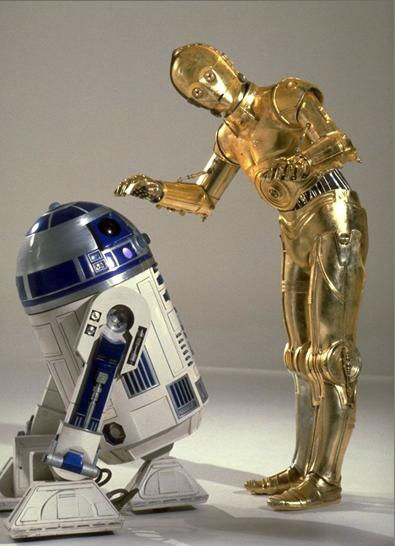
\includegraphics[width=0.8 \linewidth, height=0.8 \textheight, keepaspectratio]{images/c3po_r2d2}
		\end{minipage}%
		\begin{minipage}{.33\textwidth}
				\begin{minipage}{\textwidth}
			  \phantom{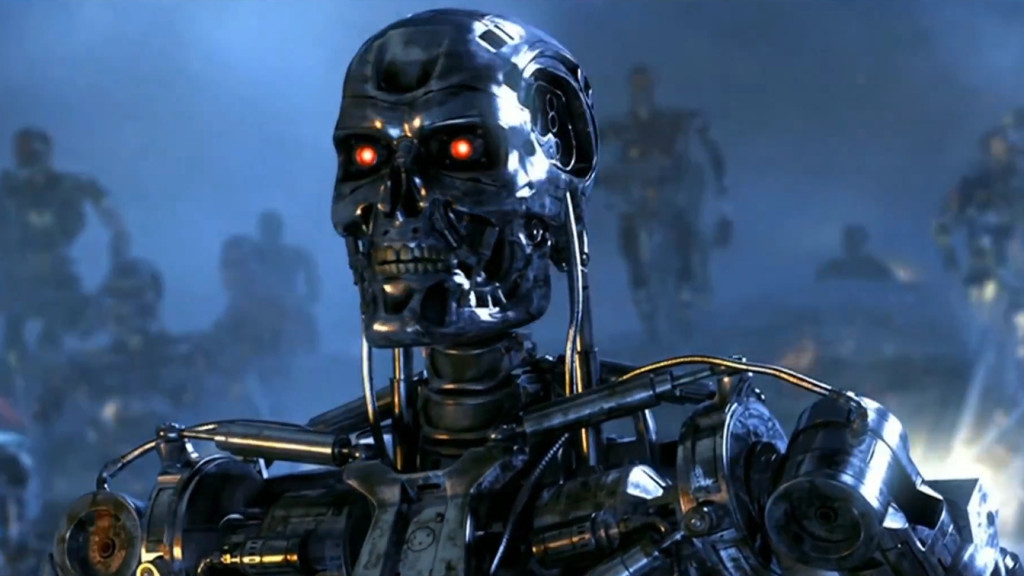
\includegraphics[width=0.8 \linewidth, height=0.8 \textheight, keepaspectratio]{images/terminator}}
			\end{minipage}
			\begin{minipage}{\textwidth}
			  \phantom{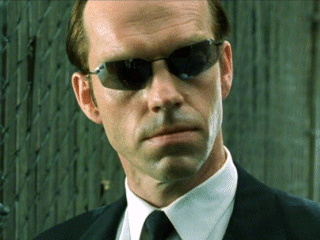
\includegraphics[width=0.8 \linewidth, height=0.8 \textheight, keepaspectratio]{images/smith}}
			\end{minipage}
		\end{minipage}%
		\begin{minipage}{.33\textwidth}
		  \phantom{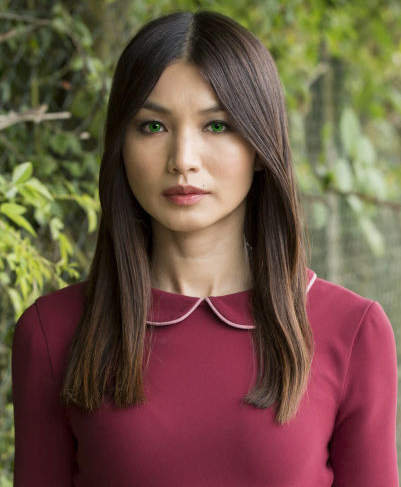
\includegraphics[width=0.8 \linewidth, height=0.8 \textheight, keepaspectratio]{images/mia}}
		\end{minipage}
	\end{figure}
\end{frame}

\begin{frame} {SciFi AI}
	\begin{figure}
		\centering
		\begin{minipage}{.33\textwidth}
		  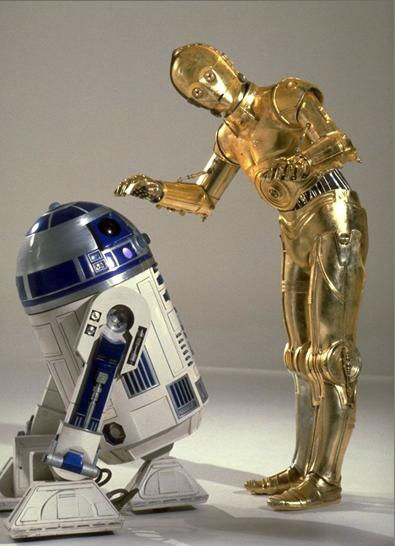
\includegraphics[width=0.8 \linewidth, height=0.8 \textheight, keepaspectratio]{images/c3po_r2d2}
		\end{minipage}%
		\begin{minipage}{.33\textwidth}
				\begin{minipage}{\textwidth}
			  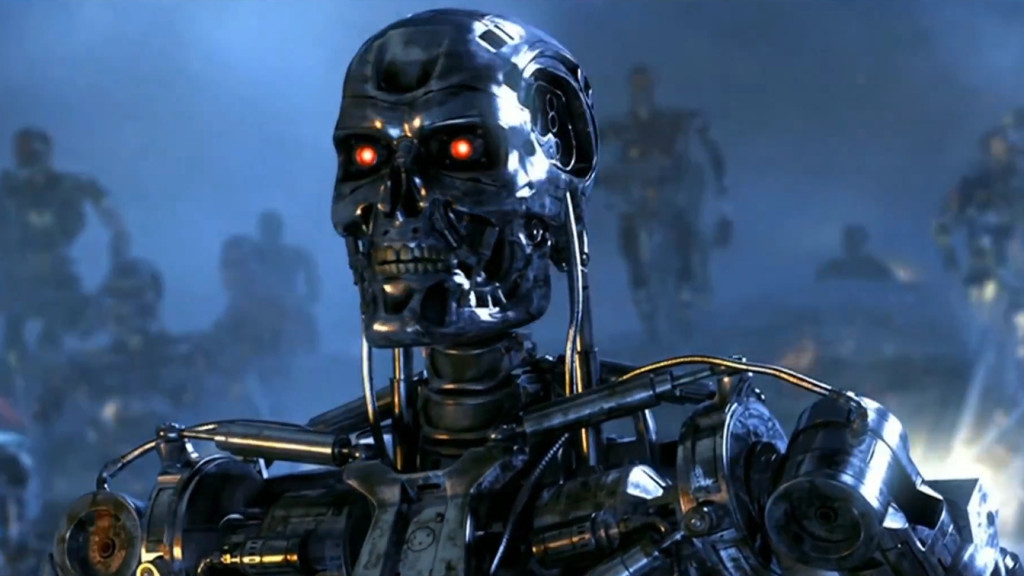
\includegraphics[width=0.8 \linewidth, height=0.8 \textheight, keepaspectratio]{images/terminator}
			\end{minipage}
			\begin{minipage}{\textwidth}
			  \phantom{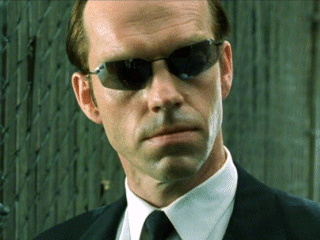
\includegraphics[width=0.8 \linewidth, height=0.8 \textheight, keepaspectratio]{images/smith}}
			\end{minipage}
		\end{minipage}%
		\begin{minipage}{.33\textwidth}
		  \phantom{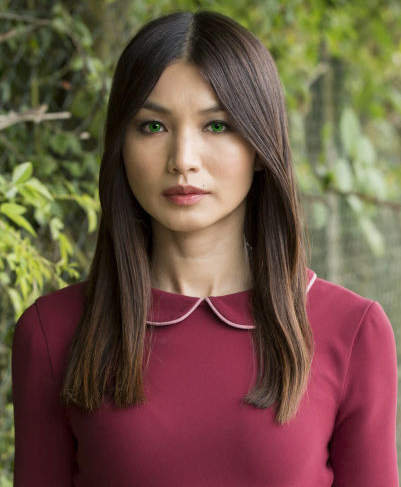
\includegraphics[width=0.8 \linewidth, height=0.8 \textheight, keepaspectratio]{images/mia}}
		\end{minipage}
	\end{figure}
\end{frame}

\begin{frame} {SciFi AI}
	\begin{figure}
		\centering
		\begin{minipage}{.33\textwidth}
		  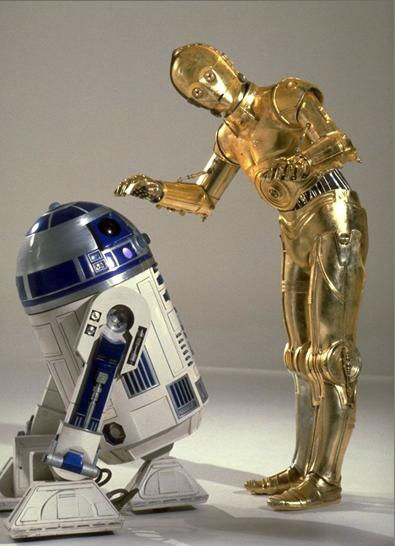
\includegraphics[width=0.8 \linewidth, height=0.8 \textheight, keepaspectratio]{images/c3po_r2d2}
		\end{minipage}%
		\begin{minipage}{.33\textwidth}
				\begin{minipage}{\textwidth}
			  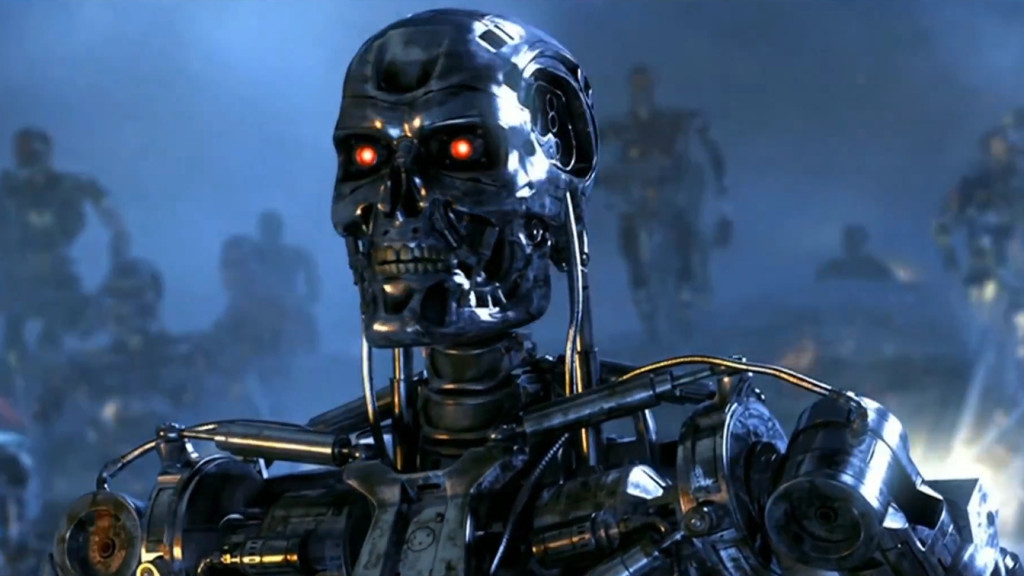
\includegraphics[width=0.8 \linewidth, height=0.8 \textheight, keepaspectratio]{images/terminator}
			\end{minipage}
			\begin{minipage}{\textwidth}
			  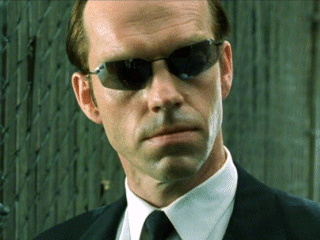
\includegraphics[width=0.8 \linewidth, height=0.8 \textheight, keepaspectratio]{images/smith}
			\end{minipage}
		\end{minipage}%
		\begin{minipage}{.33\textwidth}
		  \phantom{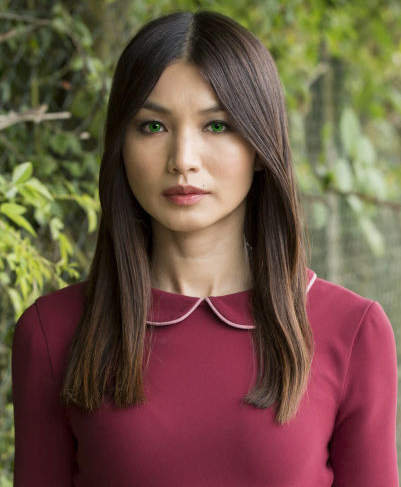
\includegraphics[width=0.8 \linewidth, height=0.8 \textheight, keepaspectratio]{images/mia}}
		\end{minipage}
	\end{figure}
\end{frame}

\begin{frame} {SciFi AI}
	\begin{figure}
		\centering
		\begin{minipage}{.33\textwidth}
		  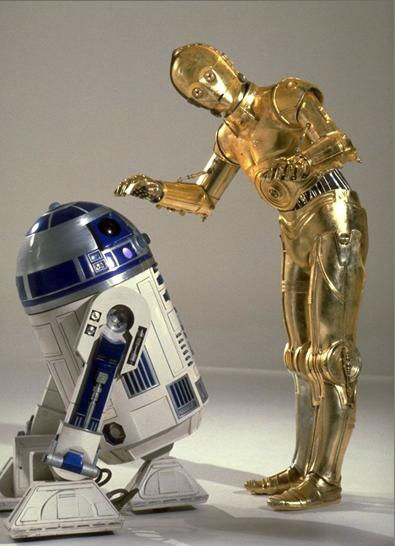
\includegraphics[width=0.8 \linewidth, height=0.8 \textheight, keepaspectratio]{images/c3po_r2d2}
		\end{minipage}%
		\begin{minipage}{.33\textwidth}
				\begin{minipage}{\textwidth}
			  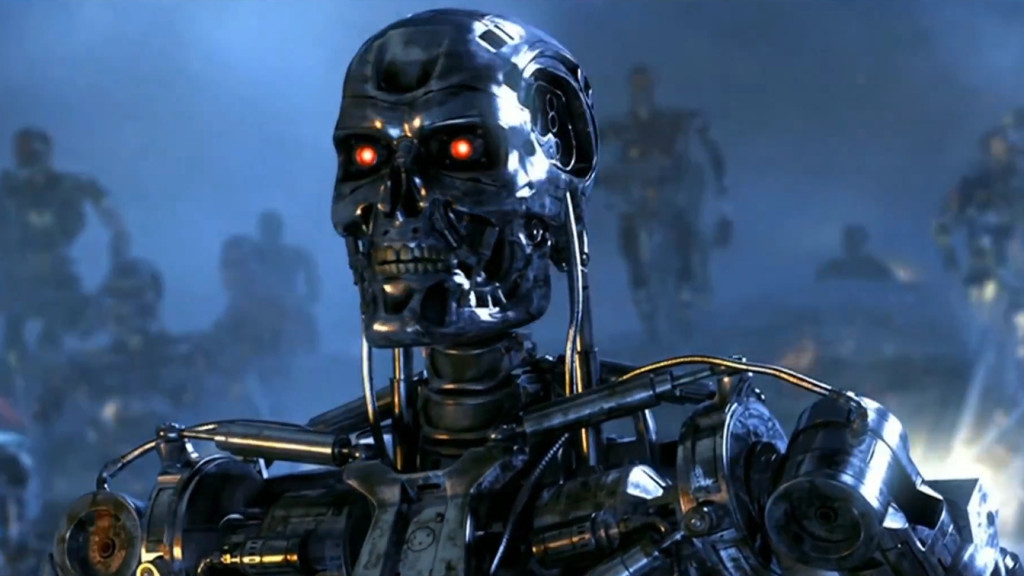
\includegraphics[width=0.8 \linewidth, height=0.8 \textheight, keepaspectratio]{images/terminator}
			\end{minipage}
			\begin{minipage}{\textwidth}
			  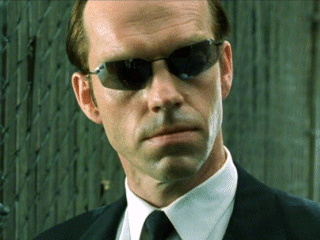
\includegraphics[width=0.8 \linewidth, height=0.8 \textheight, keepaspectratio]{images/smith}
			\end{minipage}
		\end{minipage}%
		\begin{minipage}{.33\textwidth}
		  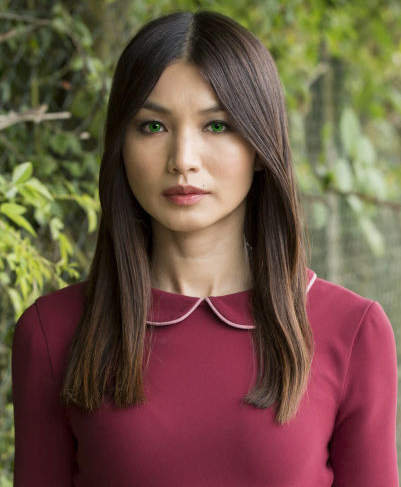
\includegraphics[width=0.8 \linewidth, height=0.8 \textheight, keepaspectratio]{images/mia}
		\end{minipage}
	\end{figure}
\end{frame}

\section{Разделы AI}

\begin{frame}{Разделы AI}
  \centering
  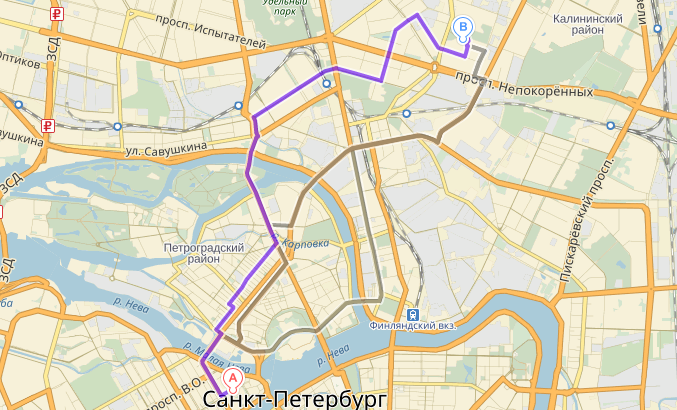
\includegraphics[width=0.8 \linewidth, height=0.8 \textheight, keepaspectratio]{images/maps}\\
	Анализ графов
\end{frame}

\begin{frame}{Разделы AI}
  \centering
  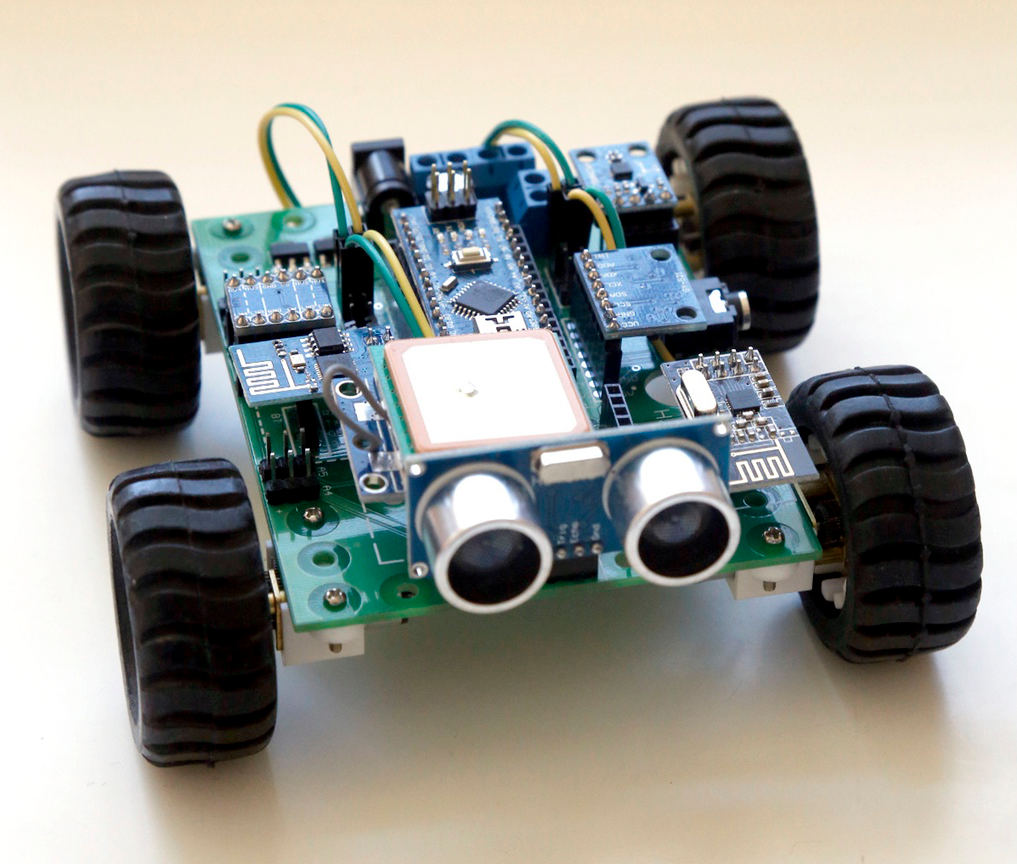
\includegraphics[width=0.8 \linewidth, height=0.8 \textheight, keepaspectratio]{images/robot}\\
	Робототехника
\end{frame}

\begin{frame}{Разделы AI}
	\begin{itemize}
	  \item[--] Работа с естественными языками
		\item[--] Представление и использование знаний
		\item[--] Компьютерное зрение
		\item[--] Машинное обучение
		\item[--] Биологическое моделирование искусственного интеллекта
		\item[--] Робототехника
		\item[--] \ldots
	\end{itemize}
\end{frame}

\section{В чем отличия ML от AI?}

\begin{frame}{Что такое машинное обучение?}
	Arthur Samuel (1959). \\
	\bigbreak
	Field of study that gives computers the ability to learn without being explicitly programmed.
\end{frame}

\begin{frame}{Пример}
  Чем отличается задача “найти кратчайший путь в графе” от “антиспам фильтр”?
\end{frame}

\begin{frame}{Что такое машинное обучение?}
	Tom Mitchell (1998) \\
	\bigbreak
	Well-posed Learning Problem: A computer program is said to learn from experience E with respect to some task T and some performance measure P, if its performance on T, as measured by P, improves with experience E\\
	\bigbreak
	E.g., Learn to play checkers\\ 
	\bigbreak
	T : Play checkers\\
	P : \% of games won in world tournament\\
	E : opportunity to play against self\\
\end{frame}

\section{Где используется ML}

\begin{frame}{Где используется ML?}
	\begin{itemize}
	  \item[--] Рекомендации на Amazon, Kinopoisk
	  \item[--] Поисковые системы Google, Яндекс
	  \item[--] Выделение лиц друзей на фото Facebook
	  \item[--] Боты в Twitter
	\end{itemize}
\end{frame}

\section{Какая математика понадобится}

\begin{frame}{Какая математика понадобится?}
	\begin{itemize}
	  \item[--] Математическая статистика 
	  \item[--] Методы оптимизации 
	  \item[--] Дискретная математика
	  \item[--] Теория вероятности
	  \item[--] Линейная алгебра
	\end{itemize}
\end{frame}

\section{Кто уже использовал методы машинного обучения? }

\section{Достаточно ли знать алгоритмы ML и математику?}

\begin{frame}{Что еще надо понимать}
	\begin{itemize}
	  \item[--] Когда надо применять ML
	  \item[--] Как сформулировать задачу в терминах ML
	  \item[--] Как выбрать подходящий класс алгоритмов
	  \item[--] Где посмотреть существующие решения
	  \item[--] Как настроить алгоритм
	  \item[--] Как оценить результаты
	\end{itemize}
\end{frame}

\section{Немного истории}

\begin{frame}{Тест Тьюринга}
    AI как наука начался с теста Тьюринга (1950).\\
    \bigbreak
    Компьютер должен успешно выдать себя за человека в (письменном) диалоге между судьёй, человеком и компьютером
\end{frame}

\begin{frame}{История ML}
	\begin{itemize}
	  \item[--] 50-70 гг. -- Базы знаний, полнотекстовый поиск, распознавание образов, нейронные сети, К ближайших соседей.
	  \item[--] 1973г. -- “Зима” искуственного интеллекта
	  \item[--] 80-90гг.  -- Первые конференции, развитие практического применения
	  \item[--] 90-00гг. -- Метод опорных векторов, бустинг
	  \item[--] Рандомизированный решающий лес (начало 2000х)
	  \item[--] Обучение Марковских случайных полей (2000е)
	  \item[--] Глубокое обучение (2006)
	\end{itemize}
\end{frame}

\begin{frame}{Зима AI}
	\begin{itemize}
	  \item[--] Проблема комбинаторного взрыва
	  \item[--] Низкая производительность компьютеров
	  \item[--] Проблема представлений знаний “здравого мысла”
	  \item[--] Парадокс Моравеца
	\end{itemize}
\end{frame}

\section{Типы Машинного Обучения}

\begin{frame}{Типы машинного обучения}
	\begin{itemize}
	  \item[--] С учителем
	  \item[--] Без учителя
	  \item[--] Смешанное
	\end{itemize}
\end{frame}

\begin{frame}{Обучение с учителем. Классификация}
  \TODO {picture}
\end{frame}

\begin{frame}{Обучение с учителем. Регрессия}
  \TODO {picture}
\end{frame}

\begin{frame}{Обучение с учителем }
	Множество объектов $X$ \\
	Множество допустимых ответов $Y$\\
	Обучающая выборка - совокупность пар ${X^l = (x_i,y_i)_{i=1}^l}$ \\
	Целевая функция ${y^*:X \rightarrow Y}$\\
	\bigbreak
	\alert{Задача}:\\
	Найти решающую функцию ${a: X \rightarrow Y}$  \\
	Решающая функция должна приближать целевую на всем множестве ${X}$
\end{frame}

\begin{frame}{Обучение с учителем}
  \TODO {пример}
\end{frame}

\begin{frame}{Обучение с учителем }
	\begin{itemize}
	  \item[--] Классификация (${Y={1,2,..,K}}$ конечно) — множество $X$ разбивается на $K$ классов. Требуется предсказать к какому классу он принадлежит. 
	  \item[--] Восстановление регрессии ${(Y=\mathbb{R})}$ — требуется найти функцию $f$ из определенного класса, которая аппроксимирует $f^*$
	\end{itemize}
\end{frame}

\section{Обучение без учителя}

\begin{frame}{Обучение без учителя}
  \TODO {пример}
\end{frame}

\begin{frame}{Типы признаков}
	${f: X \rightarrow D_f}$
	\begin{itemize}
	  \item[--] Бинарные (${D_f = \left\{ 0, 1 \right\} }$)
	  \item[--] Номинальные (${D_f}$ -- конечное множество)
	  \item[--] Порядковые (${D_f}$ -- конечное упорядоченное множество)
	  \item[--] Количественные (${D_f = \mathbb{R} }$)
	\end{itemize}
\end{frame}

\begin{frame}{Типы признаков (примеры)}
	\begin{itemize}
	  \item[--] Бинарные (Пол, наличие боли в спине, в сознании ли пациент)
	  \item[--] Номинальные (Тип боли: колющая, режущая, ноющая)
	  \item[--] Порядковые (Общее состояние больного: удовлетворительное, средней тяжести, тяжелое, крайне тяжелое)
	  \item[--] Количественные (Температура тела, пульс, артериальное давление)
	\end{itemize}
\end{frame}

\begin{frame}{Применение ML}
	\begin{itemize}
	  \item[--] Академическое\\
	Красивые идеи, хорошая математика
	  \item[--] Практическое\\
	  Обеспечивает некоторое качество на множестве примеров\\
	\end{itemize}
\end{frame}

\begin{frame}{Что читать/смотреть}
  \href{http://www.machinelearning.ru/wiki/images/6/6d/Voron-ML-1.pdf}{Курс К. В. Воронцова}\\
	\href{https://yandexdataschool.ru/edu-process/courses/machine-learning}{Видеолекции ШАД}\\
	Christopher M. Bishop "Pattern Recognition and Machine Learning"
	G. James, D. Witten, T. Hastie, R. Tibshirani: "An Introduction to Statistical Learning" 	
\end{frame}

\begin{frame}{На следующей лекции}
	\begin{itemize}
	  \item[--] Метод ближайших соседей
	  \item[--] Гипотеза компактности
	  \item[--] Обобщенный метрический классификатор
	  \item[--] Проклятие размерности  
	  \item[--] Отбор эталонов     
	\end{itemize}
\end{frame}

\end{document}